\documentclass[10pt]{article}

\usepackage[T1]{fontenc}
\usepackage{lmodern}
\usepackage[margin=0.68in]{geometry}
\usepackage{amsmath}
\usepackage{graphicx}
\usepackage{booktabs}
\usepackage{tabularx}
\usepackage{array}
\usepackage{float}
\usepackage{microtype}
\usepackage{enumitem}
\usepackage[hidelinks]{hyperref}
\usepackage{xcolor}
\usepackage{fancyhdr}

\newif\ifshowedit
\showeditfalse

\definecolor{reportblue}{HTML}{174A6E}
\definecolor{reportred}{HTML}{8F2828}
\newcolumntype{Y}{>{\raggedright\arraybackslash}X}
\setlist{nosep,leftmargin=*}
\setlength{\emergencystretch}{2em}
\setlength{\parindent}{0pt}
\setlength{\parskip}{3pt}
\setlength{\headheight}{13pt}
\pagestyle{fancy}
\fancyhf{}
\lhead{\small arXiv Primary-Category Classification}
\rhead{\small Gary Zhang \quad \thepage}
\renewcommand{\headrulewidth}{0.35pt}
\hypersetup{
  colorlinks=true,
  linkcolor=reportblue,
  urlcolor=reportblue,
  pdftitle={Classifying 112 arXiv Primary Categories from Titles and Abstracts},
  pdfauthor={Gary Zhang}
}

\title{\vspace{-2.1em}\textbf{Classifying 112 arXiv Primary Categories\\
from Titles and Abstracts}}
\author{Gary Zhang \qquad AI Bootcamp}
\date{July 30, 2026}

\begin{document}
\maketitle
\vspace{-1.7em}

\section{Project question and current status}

This project asks whether a small neural classifier can predict one paper's
author-selected arXiv \texttt{primary\_category} from its title and abstract.
Reliable routing could support search or dataset organization, but a predicted
category is not proof of a paper's scientific identity. I completed data
curation, duplicate checks, a train-validation-test pipeline, current-model
retraining, held-out evaluation, and error inspection using the course
classification workflow \cite{course}. Current blocker is sample size: the
median category has only four held-out papers, so rare-category estimates
remain unstable.

\subsection{Data, labels, and split}

The arXiv export API returned 11,070 submissions from July 3--15, 2026 UTC
using daily \texttt{submittedDate} queries \cite{arxivapi}. Curation removed
3,319 records. Deterministic ranking by withdrawal markers, abstract depth,
publication fields, title length, and category tagging, with proportional
category quotas, removed 2,070; subject filtering removed 1,249 Astrophysics,
Condensed Matter, and Economics papers. The classifier kept 7,708 of the
remaining 7,751 papers in 112 categories with at least five examples and
excluded 43 papers from 17 rarer categories. Table~\ref{tab:classes} gives
every target count; codes follow arXiv's taxonomy \cite{taxonomy}.

\begin{table}[H]
  \centering
  \caption{All 112 eligible primary categories and pre-split paper counts.}
  \label{tab:classes}
  \fontsize{8.0}{8.4}\selectfont
  \setlength{\tabcolsep}{2.6pt}
  \begin{tabular}{lr lr lr lr lr}
    \toprule
    Category & $n$ & Category & $n$ & Category & $n$ & Category & $n$ & Category & $n$ \\
    \midrule
    \texttt{cs.AI} & 352 & \texttt{cs.MA} & 23 & \texttt{math.AG} & 84 & \texttt{math.RA} & 20 & \texttt{physics.ins-det} & 22 \\
    \texttt{cs.AR} & 40 & \texttt{cs.MM} & 6 & \texttt{math.AP} & 182 & \texttt{math.RT} & 39 & \texttt{physics.med-ph} & 16 \\
    \texttt{cs.CC} & 22 & \texttt{cs.MS} & 5 & \texttt{math.AT} & 17 & \texttt{math.SG} & 15 & \texttt{physics.optics} & 119 \\
    \texttt{cs.CE} & 37 & \texttt{cs.NE} & 23 & \texttt{math.CA} & 28 & \texttt{math.SP} & 7 & \texttt{physics.plasm-ph} & 47 \\
    \texttt{cs.CG} & 20 & \texttt{cs.NI} & 31 & \texttt{math.CO} & 232 & \texttt{math.ST} & 57 & \texttt{physics.soc-ph} & 32 \\
    \texttt{cs.CL} & 327 & \texttt{cs.PF} & 7 & \texttt{math.CT} & 14 & \texttt{nlin.AO} & 8 & \texttt{q-bio.BM} & 5 \\
    \texttt{cs.CR} & 205 & \texttt{cs.PL} & 25 & \texttt{math.CV} & 29 & \texttt{nlin.CD} & 7 & \texttt{q-bio.NC} & 18 \\
    \texttt{cs.CV} & 779 & \texttt{cs.RO} & 335 & \texttt{math.DG} & 69 & \texttt{nlin.PS} & 6 & \texttt{q-bio.PE} & 12 \\
    \texttt{cs.CY} & 56 & \texttt{cs.SC} & 5 & \texttt{math.DS} & 74 & \texttt{nlin.SI} & 7 & \texttt{q-bio.QM} & 16 \\
    \texttt{cs.DB} & 29 & \texttt{cs.SD} & 64 & \texttt{math.FA} & 67 & \texttt{nucl-ex} & 15 & \texttt{q-fin.CP} & 6 \\
    \texttt{cs.DC} & 65 & \texttt{cs.SE} & 203 & \texttt{math.GM} & 13 & \texttt{nucl-th} & 54 & \texttt{q-fin.GN} & 5 \\
    \texttt{cs.DL} & 14 & \texttt{cs.SI} & 16 & \texttt{math.GN} & 7 & \texttt{physics.acc-ph} & 11 & \texttt{q-fin.MF} & 7 \\
    \texttt{cs.DM} & 12 & \texttt{eess.AS} & 49 & \texttt{math.GR} & 32 & \texttt{physics.ao-ph} & 14 & \texttt{q-fin.PM} & 5 \\
    \texttt{cs.DS} & 93 & \texttt{eess.IV} & 47 & \texttt{math.GT} & 42 & \texttt{physics.app-ph} & 17 & \texttt{q-fin.ST} & 5 \\
    \texttt{cs.ET} & 11 & \texttt{eess.SP} & 121 & \texttt{math.HO} & 7 & \texttt{physics.atom-ph} & 25 & \texttt{q-fin.TR} & 9 \\
    \texttt{cs.FL} & 6 & \texttt{eess.SY} & 132 & \texttt{math.LO} & 21 & \texttt{physics.bio-ph} & 18 & \texttt{quant-ph} & 468 \\
    \texttt{cs.GR} & 16 & \texttt{gr-qc} & 144 & \texttt{math.MG} & 16 & \texttt{physics.chem-ph} & 48 & \texttt{stat.AP} & 27 \\
    \texttt{cs.GT} & 34 & \texttt{hep-ex} & 31 & \texttt{math.NA} & 142 & \texttt{physics.class-ph} & 8 & \texttt{stat.CO} & 8 \\
    \texttt{cs.HC} & 83 & \texttt{hep-lat} & 14 & \texttt{math.NT} & 124 & \texttt{physics.comp-ph} & 25 & \texttt{stat.ME} & 114 \\
    \texttt{cs.IR} & 67 & \texttt{hep-ph} & 178 & \texttt{math.OA} & 13 & \texttt{physics.ed-ph} & 8 & \texttt{stat.ML} & 61 \\
    \texttt{cs.IT} & 76 & \texttt{hep-th} & 157 & \texttt{math.OC} & 143 & \texttt{physics.flu-dyn} & 71 & & \\
    \texttt{cs.LG} & 681 & \texttt{math-ph} & 40 & \texttt{math.PR} & 90 & \texttt{physics.geo-ph} & 11 & & \\
    \texttt{cs.LO} & 37 & \texttt{math.AC} & 29 & \texttt{math.QA} & 17 & \texttt{physics.hist-ph} & 5 & & \\
    \bottomrule
  \end{tabular}
\end{table}

\vspace{-2pt}
Each example uses only title plus abstract; its label is the single
\texttt{primary\_category}. A seed-42 per-class stratified split produced
5,394 training, 1,157 validation, and 1,157 held-out test papers. All 7,751
base arXiv IDs were unique, so no revision crossed splits. The category field,
directory names, authors, and secondary categories never entered features.

\clearpage

\section{Approach}
\subsection{Input representation}

Title and abstract are joined with two newlines. A scikit-learn
\texttt{FeatureUnion} fitted on training text only creates 8,000 TF--IDF
features \cite{sklearn}: 6,000 English word unigram/bigram features and 2,000
within-word character 3--5-gram features. Both use sublinear term frequency;
both lowercase and require two training documents per term. Word features
remove English stop words, strip Unicode accents, and discard terms appearing
in over 99.5\% of training papers. Validation and test text use the frozen
training vocabulary. The sparse matrix becomes a dense 8,000-value
\texttt{float32} tensor.

\subsection{Classifier, training, and baseline}

The PyTorch model, trained from scratch, maps 8,000 inputs to 384 ReLU hidden
units, applies dropout 0.25, and emits 112 raw logits. It has 3,115,504
trainable parameters. Square-root inverse-frequency class weights enter
cross-entropy loss, which accepts unnormalized logits \cite{pytorchloss}.
AdamW used learning rate 0.001 and weight decay 0.0001. Training used CPU,
batch size 128, seed 42, and at most 20 epochs in PyTorch 2.13.0 with
scikit-learn 1.9.0. Validation macro-F1 selected epoch 18; patience was four.
The comparison baseline always predicts training-majority class
\texttt{cs.CV}.

\subsection{Evaluation design}

Training papers fit TF--IDF and network weights. Within the July 30 run,
validation macro-F1 selected epoch 18; final metrics were computed after
restoring that checkpoint. Test results did not select features, dropout, or
epoch within this run. A fresh CLI training run wrote a version-1 checkpoint
whose hashes bind weights to exact label order and vectorizer. The evidence
notebook reconstructed the split and independently recomputed strict metrics
from 1,157 predictions.

\subsection{Metrics}

For $N$ held-out papers, accuracy is
\[
  \mathrm{accuracy}=\frac{\text{correct predictions}}{N}.
\]
For one class, $TP$ counts correctly predicted members, $FP$ counts other
papers assigned to it, and $FN$ counts its papers assigned elsewhere. For
\texttt{cs.CV}, for example, a true \texttt{cs.CV} paper predicted
\texttt{cs.LG} is an $FN$. Precision $P=TP/(TP+FP)$, recall
$R=TP/(TP+FN)$, and $F_1=2PR/(P+R)$. Macro-F1 averages 112 class F1 scores
equally, exposing rare-class failures that accuracy can hide.

\subsection{Reproducibility and scope}

Dataset SHA-256 is
\texttt{1bfe64d02fffedaaa65ef00866e47e8c688966062ba54572c404a08c4657c78a}.
The source notebook records class counts, split replay, baseline, recomputed
strict metrics, cross-list audit, two examined cases, and figure generation.
Learning curves come from the saved July 30 training artifact.

\clearpage

\section{Current results}

On 1,157 held-out papers, the classifier predicted 710 primary categories
correctly: 61.37\% accuracy, 34.65\% macro-F1, 59.15\% weighted-F1, and
84.62\% top-3 accuracy. Accuracy exceeded the majority baseline by 51.25
percentage points. Table~\ref{tab:results} also shows why accuracy alone is
insufficient: the majority rule reaches 10.11\% accuracy but only 0.16\%
macro-F1.

\begin{table}[H]
  \centering
  \caption{Strict primary-category performance on the same held-out papers.}
  \label{tab:results}
  \small
  \begin{tabularx}{\linewidth}{YcccccY}
    \toprule
    Classifier & Eval.\ $n$ & Correct & Accuracy & Macro-F1 & Top-3 & Selection \\
    \midrule
    TF--IDF MLP & 1,157 & 710 & 61.37\% & 34.65\% & 84.62\% & epoch 18 by validation macro-F1 \\
    Majority \texttt{cs.CV} & 1,157 & 117 & 10.11\% & 0.16\% & n/a & training labels only \\
    \bottomrule
  \end{tabularx}
\end{table}

\begin{figure}[H]
  \centering
  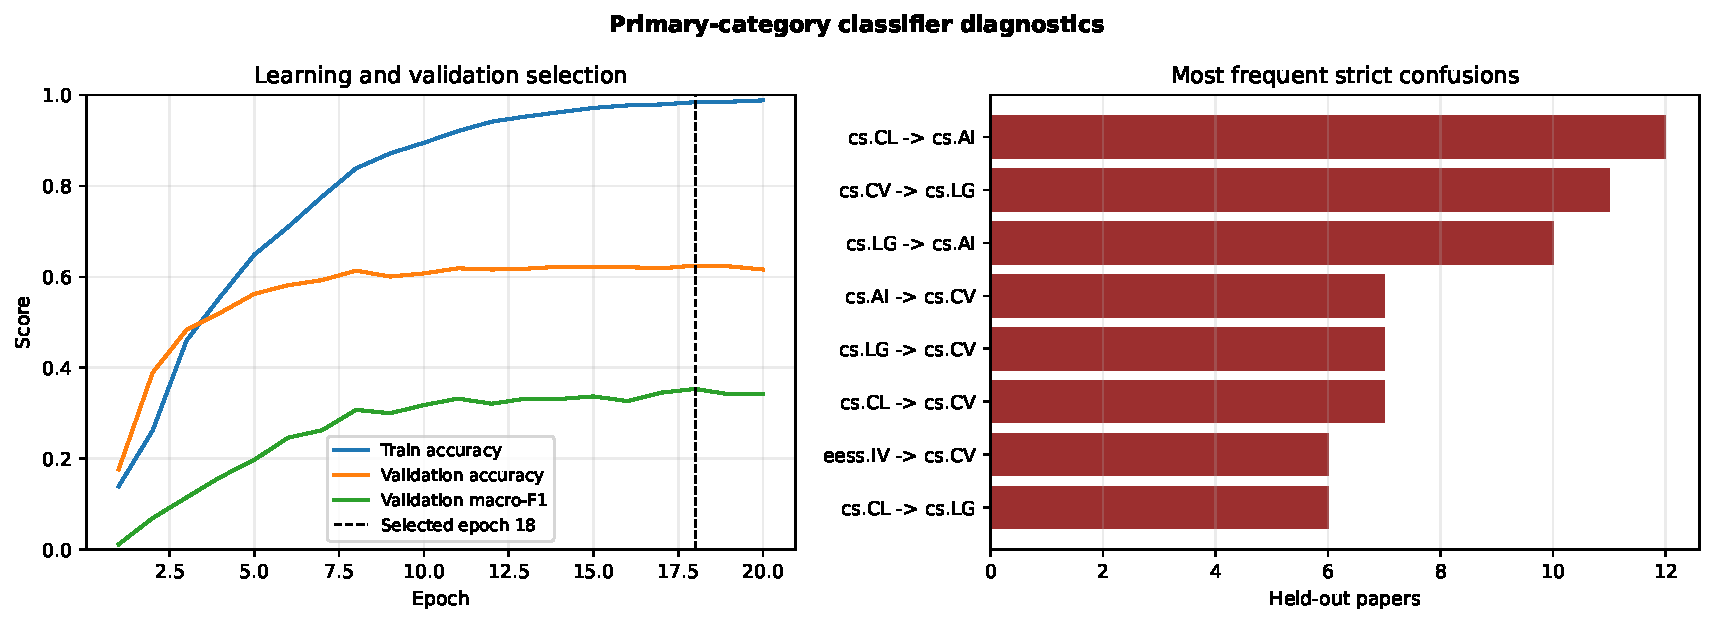
\includegraphics[width=\linewidth,height=3.15in,keepaspectratio]{results_diagnostics.pdf}
  \caption{Left: training accuracy continued toward 1.0 while validation
  accuracy and macro-F1 flattened; the dashed line marks the selected epoch.
  Right: strict primary-label errors concentrate among overlapping computing
  categories. Counts come from the 1,157-paper test set.}
  \label{fig:diagnostics}
\end{figure}

\subsection{Interpretation}

Figure~\ref{fig:diagnostics} shows a large generalization gap. At selected
epoch 18, training accuracy was 98.44\%, while validation accuracy was
62.49\% and validation macro-F1 was 35.34\%; both validation scores declined
by epoch 20. Among categories with at least ten test papers,
High Energy Physics - Phenomenology had strongest F1 (93.10\%, $n=27$);
Sound had weakest (26.67\%, $n=10$). Forty of 112 categories had zero test
F1, and 61 had four or fewer test papers. The most frequent error was
\texttt{cs.CL}$\rightarrow$\texttt{cs.AI} (12 papers), followed by
\texttt{cs.CV}$\rightarrow$\texttt{cs.LG} (11).

Primary-only scoring also hides cross-list ambiguity. A post-hoc audit, without
changing predictions, found top-1 accuracy of 70.96\% when any author-listed
category counted; 111 of 447 strict errors matched a listed secondary category.
The assignment's primary-label result remains 61.37\%. The audit indicates that
some confident disagreements reflect an intentionally narrow target.

\clearpage

\section{Error analysis}

I replayed one correct case, screened the 25 highest-confidence strict errors,
and examined two of them. Twelve screened predictions were listed secondary
categories. Table~\ref{tab:errors} shows the correct paper and two strict
errors; all three are cited because their titles and labels are discussed
\cite{dabaja,guo,buche}.

\begin{table}[H]
  \centering
  \caption{Inspected held-out predictions. Confidence is a model score.}
  \label{tab:errors}
  \small
  \begin{tabularx}{\linewidth}{>{\raggedright\arraybackslash}p{0.19\linewidth}p{0.13\linewidth}p{0.16\linewidth}Y}
    \toprule
    Paper (short title) & Primary label & Prediction & Evidence-based interpretation \\
    \midrule
    2607.09583, ``Remote Seg.'' & \texttt{cs.CV} &
    \texttt{cs.CV}, 99.95\% & Segmentation and remote-sensing image terms
    align with the primary label; this is one correct example. \\
    2607.07372, ``Quantum Control'' & \texttt{cs.AR} &
    \texttt{quant-ph}, 99.53\% & Quantum-control language dominates the title
    and abstract. \texttt{quant-ph} is also author-listed, so this is a strict
    primary-label error rather than an unrelated prediction. \\
    2607.03072, ``LOTUSim'' & \texttt{cs.MA} &
    \texttt{cs.RO}, 98.66\% & Marine-robotics vocabulary supports
    \texttt{cs.RO}, which is also author-listed. The result exposes overlap
    between primary and secondary submission labels. \\
    \bottomrule
  \end{tabularx}
\end{table}

Observed errors combine overlap and imbalance. They do not establish model
``understanding.'' Computation and Language, Artificial Intelligence, Computer
Vision, and Machine Learning share vocabulary and dominate frequent confusion
pairs. Cross-list matches explain 24.83\% of strict errors, while sparse classes
still account for many zero-F1 outcomes. These observations do not identify a
causal failure mechanism.

\section{Limitations, progress, and next step}

This is one random split from a curated 13-day window, not a chronological
forecast of future submissions. Subject-group exclusions shift the population,
and title plus abstract omits full-text evidence. Primary labels can be
cross-listed and 61 classes have at most four test papers. Dense TF--IDF tensors
also limit scale. The split protects held-out rows and duplicate base IDs, but
prior development viewed results from an earlier model on this same test
partition. The current run avoided test-based selection, but the partition is
not untouched across project history. No repeated seeds or confidence
intervals have been measured.

Next, I will change only dropout from 0.25 to 0.50 while
holding the dataset, seed-42 split, TF--IDF features, optimizer, batch size, and
epoch limit fixed. I predict a smaller train-validation gap and higher
validation macro-F1. I will decide from validation macro-F1 before reading the
new test result.

\section{Conclusion}

The classifier reached 61.37\% strict primary-category accuracy (710 of 1,157)
and 34.65\% macro-F1, beating the majority baseline by 51.25 percentage points.
This result does not establish reliable rare-class or future-paper performance.
Most important completed step is validation-selected evaluation with duplicate
and feature-leakage controls; remaining step is the dropout experiment.

\begin{thebibliography}{9}
\footnotesize
\setlength{\itemsep}{0pt}
\setlength{\parskip}{0pt}

\bibitem{course}
High School AI Bootcamp, ``Classification with PyTorch,'' course materials,
2026.

\bibitem{arxivapi}
arXiv, \emph{API User's Manual},
\url{https://info.arxiv.org/help/api/user-manual.html}, accessed July 30, 2026.

\bibitem{taxonomy}
arXiv, \emph{Category Taxonomy},
\url{https://arxiv.org/category_taxonomy}, accessed July 30, 2026.

\bibitem{sklearn}
scikit-learn developers, \emph{TfidfVectorizer documentation}, version 1.9.0,
\url{https://scikit-learn.org/stable/modules/generated/sklearn.feature_extraction.text.TfidfVectorizer.html}.

\bibitem{pytorchloss}
PyTorch contributors, \emph{CrossEntropyLoss documentation}, version 2.13.0,
\url{https://docs.pytorch.org/docs/stable/generated/torch.nn.CrossEntropyLoss.html}.

\bibitem{dabaja}
M. Dabaja and T. Celik, ``Promptable Concept Segmentation from Above:
Evaluating SAM 3's Zero-Shot and One-Shot Capabilities in Remote Sensing,''
arXiv:2607.09583, 2026.

\bibitem{guo}
X. Guo et al., ``Vectorizing Quantum Control: A RISC-V Vector Extension
Architecture for Scalable Qubit Systems,'' arXiv:2607.07372, 2026.

\bibitem{buche}
C. Buche et al., ``LOTUSim: Multi-Domain Simulator for Marine Robotics,''
arXiv:2607.03072, 2026.

\end{thebibliography}

\end{document}
